\hypertarget{Teknologier}{}
\section{Teknologier}
Grunden til vi laver en web applikation er at den nemt skal kunne integreres ude på Ordbogen A/S  og at man nemt skal kunne tilgå den.
Vi har også begge arbejdet med webudvikling i vores praktikforløb hos Ordbogen A/S, og derfor var det bekvemt for os at forsætte ad samme sti.
Derudover er det også det virksomheden primært beskæftiger sig med, så derfor synes vi denne type applikation gav mest mening til dette projekt.
\hypertarget{Laravel}{}
\subsection{Laravel}
\label{Laravel}
Vi bruger Laravels Lumen framework, der er et micro-framework lavet af Laravel. Grunden til vi valgte Lumen
fremfor Laravel, var at vi gerne ville have mere kontrol over de ting vi lavede og at Lumen bliver også brugt ude på Ordbogen.
Så hvis vi kigger på fremtidig udvikling af systemet fra Ordbogen, gav det mest mening.
Dokumentationen til Lumen er rigtig god og det gør det nemt at komme i gang med, der går ikke lang tid fra opstart
til man har noget konkret at vise. 
Derudover bygger vi vores applikation op omkring RESTful API og Lumen, har gjort det rigtig let for os at bygge 
et API op.\footnote{http://lumen.laravel.com}
\hypertarget{AngularJS}{}
\subsection{AngularJS}
Vi bruger AngularJS frameworket til vores frontend da vi begge havde arbejdet med det
i vores praktikperiode. AngularJS har nogle libraries der gør det nemt for os at tilgå de RESTful APIs
vi har lavet i backenden. 
Derudover findes der rigtig mange eksterne libraries, som ved hjælp af Angulars Dependency Injection er nemme at implementere.\footnote{https://angularjs.org/}
\hypertarget{GoogleChartAPI}{}
\subsection{Google Chart API}
Da vi bestemte os for at bruge Google Charts gjorde vi det på baggrund af det er let tilgængeligt.
Det har en god dokumentation og det bliver vedligeligholdt også kommer det fra en kilde der er garant for gode produkter.
det er meget intuitivt og tilbyder de nødvendige funtionaliteter i forhold til visning af diagrammer 
Det er også lavet til at fungere på tværs af browsere da det renderer med HTML5/SVG, 
det gør også at det eneste krav til at det skal kunne køre på klienten, er en browser.\footnote{https://developers.google.com/chart/interactive/docs/}. 
Derudover er der et angular library der gør det endnu nemmere at integrere i AngularJS.
\subsection{ElasticSearch}
Vi har anvendt ElasticSearch til at gemme data, som et alternativ til en SQL database.
\\\\
ElasticSearch er en næsten real-time search engine som er bygget på Apache Lucene, som er et søge API.\
ElasticSearch er bygget op omkring et Cluster, som er en liste af nodes, hvor en node er en server der gemmer data. Cluster indekserer så dataen og gør det søgbart\footnote{https://www.elastic.co/guide/en/elasticsearch/reference/current/setup-repositories.html}.
ElasticSearch gør også brug af index, som er en liste af dokumenter, der har samme karakteristika og er skrevet i JSON format.
\\
Ved større index kan de dele et index op i shards og et shard er et fuldt funktionelt index. Det gør man kan skalere data horisontalt.
\\\\
Vi har på figur~\ref{fig:elasticsearch-arkitektur} forsøgt at skitsere den generelle opbygning af en typisk ElasticSearch server, og relationer mellem cluster, nodes og dokumenter.
\\\\
\begin{figure}[H]
    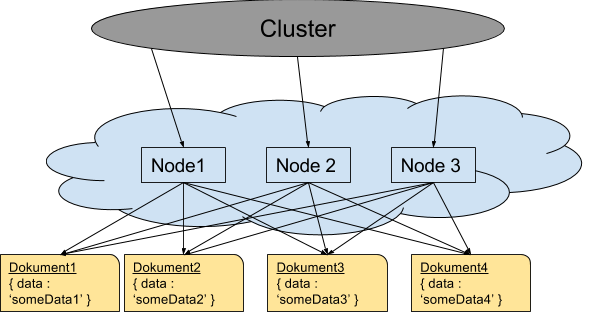
\includegraphics[scale=0.7]{ElasticSearch_arkitektur}
    \caption{Skitsering af ElasticSearch}
    \label{fig:elasticsearch-arkitektur}
\end{figure}
\subsection{Problemstilling omkring håndtering af data}
Vi har en problemstilling der går på at vi skal have noget data ind i vores ElasticSearch database, for at kunne præsentere det.
Problemstillingen går på, om vi skal pulle data ud fra de API'er der bliver tilgængelige for vores system. Eller om de forskellige teams der uploader API'er selv skal stå for at pushe data ind til vores database.
\\\\
Fordele og ulemper ved de forskellige løsninger er vigtige i forhold til hvordan systemet skal bygges op.
Vi har nedskrevet nogle overordnede fordele og ulemper for de to forskellige løsninger.
\\\\
\textbf{Fordele ved pull af data}
\begin{itemize}
    \item{Vi har selv styr på hvilke data vi henter}
    \item{Vi vælger selv hvornår data skal hentes}
    \item{Vi kan nemmere kontrollere hvor meget data der bliver hentet ind}
    \item{Hvis serveren er nede mister vi ikke data, da vi selv bestemmer hvornår vi henter data ind}
\end{itemize}
\textbf{Ulemper ved pull af data}
\begin{itemize}
    \item{Vi står selv for at hente data ind}
\end{itemize}
\textbf{Fordele ved at pushe data}
\begin{itemize}
    \item{Det er ikke os der skal stå for at hente data}
\end{itemize}
\textbf{Ulemper ved at pushe data}
\begin{itemize}
    \item{Vi kan ikke bestemme hvilke data eller hvor meget der bliver uploadet}
    \item{Hvis vores server er nede når der bliver pushet mister vi data}
    \item{Der skal lægges meget tid i at skalere data der kommer ind}
\end{itemize}
Ud fra fordele og ulemper ved begge løsninger har vi valgt at gå videre med pull af data, da det vigtigste for os bliver at vi selv kan kontrollere hvordan vi vil skalere vores data. Herudover giver det os nogle fordele når vi selv kan udvælge hvilke data vi gerne vil have ind på vores cluster. Dette vil gøre at vi skal arbejde lidt mere med hvordan vi håndterer data fra de forskellige API'er, men vi har vurderet at det er det værd i forhold til systemet.
